\documentclass{article}
\usepackage{graphicx} % Required for inserting images
\usepackage{amsfonts}
\usepackage{siunitx} 
\title{24.12.31 Index Check Benchmark}
\author{Xun Zhang \quad \quad Wuyun Siqin \quad \quad Bingsheng Zhang \\ 
Zhejiang University, CHN \\
22221024@zju.edu.cn \quad 3210101763@zju.edu.cn \quad bingsheng@zju.edu.cn}
\date{December 31 2024}

\begin{document}

\maketitle

\section{Relations and Circuit}

The index check circuit is designed to prove the following relation:

\begin{itemize}
    \item $\forall i : \mathsf{index}_i \leq m$ and $\forall i \neq j : \mathsf{index}_i \neq \mathsf{index}_j$.

\end{itemize}

Where $m$ is the total number of lottery. Each signer's lottery index should be less than total number, and there can not be two same lottery numbers of different signers. This index will be used in the eligibility check(as a input of mapping/hash function).


Our circuit implementation includes a compare gate for $\mathsf{index}_i$ and $m$, and also many gates for inequality check between every $\mathsf{index}_i$.

The code is like bellowing:

\vspace{0.5cm}

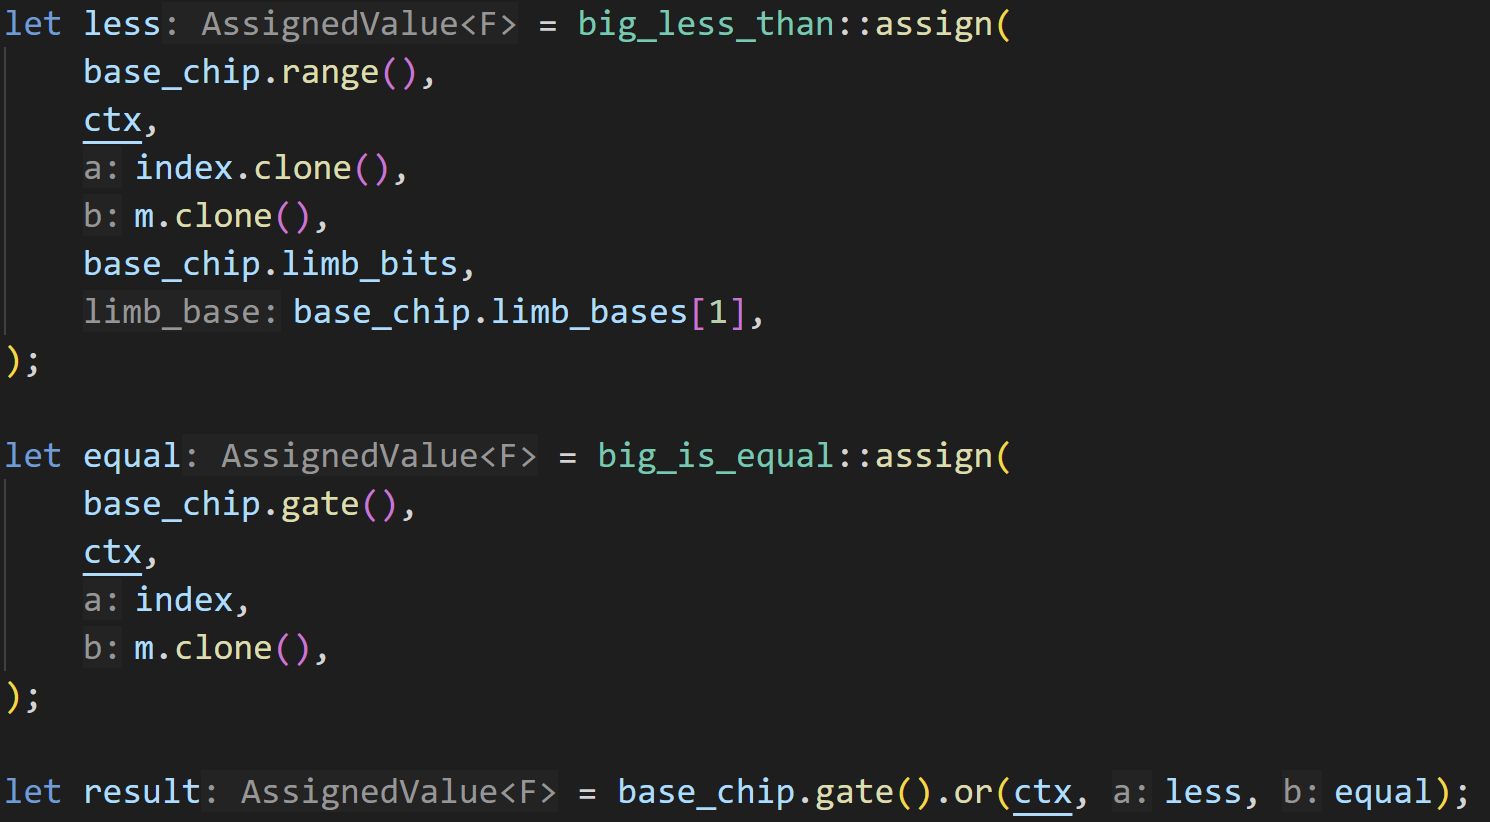
\includegraphics[width=1\linewidth]{index_check_code1.png}

This two gates is same as eligibility check gate, compare the index with $m$.

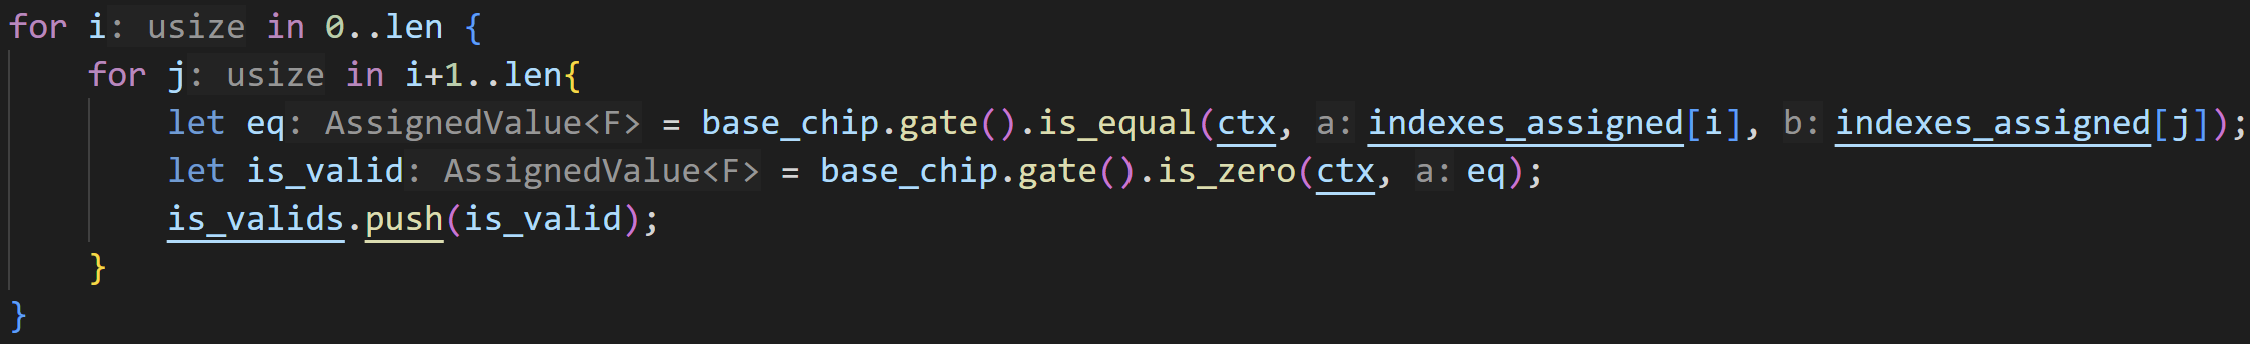
\includegraphics[width=1\linewidth]{index_check_code2.png}

This code compares each index pairwise, and constraint it to unequal.


\section{Benchmark}

The benchmark setting is $num\_limbs = 3$, and $limb\_bits = 90$.

Here is our index check benchmark result:


\begin{table}[htbp]
  \centering
    \begin{tabular}{|c|c|c|c|c|c|}
    \hline
    {Degree} & {Advice} & {Number} & {Proof Time} & {Proof Size} & {Verify Time} \\
    \hline
    18 & 1 & 128 & 5.2626s & 960 & 6.8613ms \\ \hline
    18 & 1 & 256 & 8.1488s & 1920 & 8.3849ms \\ \hline
    18 & 1 & 512 & 15.9302s & 4576 & 8.1831ms \\ \hline
    18 & 48 & 1024 & 44.1102s & 14944 & 12.5294ms \\ \hline
    20 & 48 & 2048 & 182.2723s & 14944 & 13.2670ms \\
    \hline
  \end{tabular}
  \caption{Index Check Benchmark}
\end{table}

Due to our circuit implementation, the proving cost of index check is $O(n^2)$, where $n$ is the number of indexes.


\section{Parameters}

We can find the parameters in the Mithril paper:

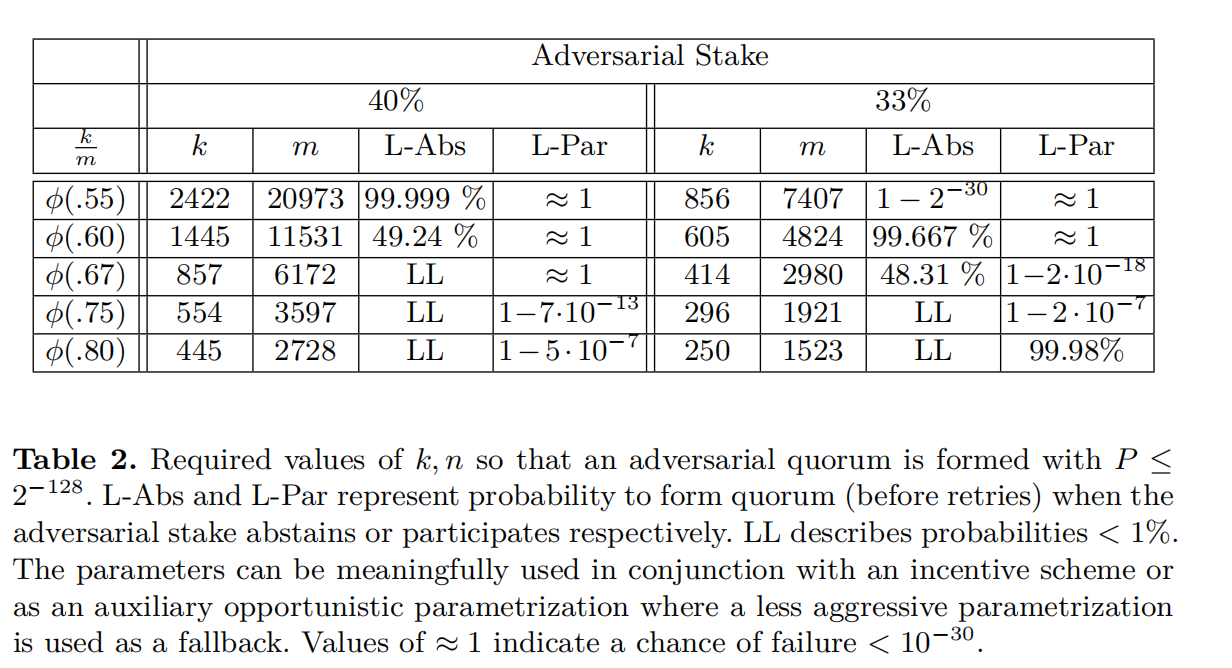
\includegraphics[width=1\linewidth]{mithril_km_parameter.png}

The recommend parameters is around hundreds, so this part is not so expensive, although it is a super-linear proving task.


\end{document}
